% \documentclass[twocolumn]{article}
\documentclass{article}
\usepackage[utf8]{inputenc}
\usepackage{hyperref}
\usepackage{titling}
\usepackage{graphicx}
\usepackage{caption}
\usepackage{subcaption}
\usepackage{multicol}
\setlength{\columnsep}{5mm}
\usepackage{geometry}
 \geometry{
 a4paper,
 total={170mm,257mm},
 left=20mm,
 top=20mm,
 }
 \usepackage{booktabs}
 \newenvironment{Figure}
  {\par\medskip\noindent\minipage{\linewidth}}
  {\endminipage\par\medskip}

% \setlength{\droptitle}{-10em} 

\title{Predicting NFL Game Outcomes}
\author{Michael Nercessian, Rohan Lewis, and Matthew Armstrong}
\date{December 13, 2020}


\begin{document}
% \twocolumn
\maketitle

\begin{multicols}{2}

\section{Introduction}

With 16-game long regular seasons, team rosters of over 50 players, and hundreds of injuries per season, NFL games are difficult to predict. The outcome of a football game is highly dependent on individual performance during that game, further increasing its unpredictability. Nonetheless, football is without a doubt the most popular betting sport in the USA, and comprises approximately \$100 billion wagered at offshore sports books\footnote{\href{https://www.legalsportsbetting.com/how-much-money-do-americans-bet-on-sports/}{\underline{Legal Sports Betting}} }. Our project aims to predict the point differential of NFL games with the ultimate goal of predicting a more accurate point spread than Vegas lines.

For each game, Vegas sets a point spread, or line, by which it is expected the favorite team will win. For example, Vegas may set a line of -4 for the Buffalo Bills over the New England Patriots, which corresponds with an expected outcome of the Bills winning by 4 points. Sports bettors can place bets on either side of this line and profit if they are correct. For example, a bettor who expects the Bills to win by more than 4 points would bet on the Bills with a -4 line, and would profit if the Bills win. On the other hand, a fan could bet on the Patriots with a +4 line, and they would profit if the Patriots win, or if the Bills win by 3 or fewer points. Payouts are structured in such a way that at the end of the day, Vegas will always profit if their line is able to attract equal money on either side. 

Vegas has a plethora of its own models and endless data at its disposal which it uses to set its opening lines. Consistently out-predicting these lines is the endless pursuit of sports bettors. One notable caveat is that Vegas takes a “vig” off bets to ensure profits, which means the payout for a bet is slightly less than the amount a bettor risks. In numerical terms, if you place a \$110 dollar bet you will receive \$100 if you win. Through some basic algebra it follows that a bettor must win 52.4\% of bets to break even.

Vegas guarantees a profit if they are able to attract equal money to both sides of the line. For example, Vegas might attract \$11,000 in bets for the Bills side of the line, and \$11,000 for the Patriots side of the line. If the Bills win by more than 4 points, Vegas will pay out \$10,000 to the Bills bettors and pull in \$11,000 from the Patriots betters for a net profit of \$1,000, or 4.5\% of the total money placed on the game. It is therefore in the best interest of Vegas to set a line that will attract equal money to both sides of the bet; if this is accomplished, Vegas guarantees a 4.5\% profit no matter the outcome. To do this, Vegas lines shift in accordance with which side of the line bets are placed. If every bettor picks the Bills to win by more than 4, the line may shift to -5 or -6 to attract more bettors to the Patriots. In doing so, Vegas effectively hedges risk against either outcome. Shifting the line to maximize bets on either side is an overall profitable strategy, but it has the potential to reduce the accuracy in predicting the actual outcome of the game. The line is no longer carefully calibrated to predict the true outcome, but instead to attract equal money on both sides. This opens an opportunity for a precise model that can predict true outcomes better than the Vegas line to be extremely profitable. In this project, we seek to build such a model.

\section{Data Preparation}
\subsection{Data Collection}
We initially approached this problem by considering a variety of different datasets including game-by-game and play-by-play data. We decided that accumulated game-by-game data would be a more accurate predictor of a game’s outcome than play-by-play data, which we felt was too noisy. After pulling 2019 regular season game-by-game data from Pro Football Reference\footnote{\href{https://www.pro-football-reference.com/teams/buf/2019.htm}{\underline{Pro Football Reference}} } (PFR) and running initial analysis on this dataset it was clear we needed to use considerably more data as there are only 256 games in a season. In order to avoid the manual team-by-team data aggregation we needed to do for this 2019 data, we built a Python script to scrape all of the necessary game-by-game team statistics from PFR for regular season games between the years of 2002 and 2019 for a total of 4,608 games.

Additionally, we used a dataset containing the Vegas lines for all of these games, which we used as a point of comparison of our predictions and evaluation of our model’s performance.\footnote{\href{ https://www.kaggle.com/tobycrabtree/nfl-scores-and-betting-data}{\underline{NFL Scores and Betting Data}} }

\subsection{Cleaning the Data}
For the 2019 dataset, we gathered 32 CSV files, one for each NFL team, from the “Schedule & Game Results” section of the 2019 season page on PFR (example link \href{https://www.pro-football-reference.com/teams/buf/2019.htm}{\underline{here}}). We then compiled these datasets and removed duplicate games to produce our 2019 game-by-game dataset.

Once we realized we needed much more data, we devised a more clever way to collect the data as downloading the CSV files one-by-one was a cumbersome process. We wrote a Python script which allowed us to automatically scrape all the required datasets from PFR and compile them into one dataset containing all games from 2002 to 2019. We also added a unique identifier for each game which was a useful key for maneuvering our datasets. A preliminary investigation into the data led us to drop some unnecessary columns and rows from the dataset. We removed the ‘Expected Points’ columns which represent PFR’s advanced statistics for offense, defense, and special teams, as we wanted to use only raw statistics for our model, not advanced statistics built by a different model. We also removed game start times and day of the week as we did not feel these would influence whether our prediction should favor either team. 

Next, we needed to deal with all the missing data. We found entire rows of missing data where teams had bye weeks, so these rows were removed. In addition, we modified the home/away column, which contained missing values for home games, to a binary encoding in order to keep track of where a team played in a given week. We also found that entries in the turnovers and passing yards columns were missing if a team had no turnovers or passing yards in a game, so we substituted missing values with zero in these columns. We lastly added a numeric identifier for each home and away team, rather than a String value of the teams name, to avoid error down the road in misspellings and changing team names (Oakland Raiders to Los Angeles Raiders, for example).

\subsection{Feature Selection and Engineering}
Our input space contained relevant statistics for the two teams prior to that game, while our output space was the point differential of a game with positive values corresponding to a victory for the home team. We needed to structure the data so that each row would represent a game between two teams. Importantly, the columns would only consist of data from prior games as this is all that is available at the time of prediction. Our objective was to transform the game-by-game data into running season averages for each of the features in the dataset necessary for prediction.

We first constructed the Season Average Only (SAO) dataset, with a feature space containing the information over all games from 2002 to 2019. We created 22 features for prediction, which were the following 11 statistics for both home and away team: win percentage, points per game, first downs per game, rushing yards per game, passing yards per game, turnovers per game, points allowed per game, first downs allowed per game, rushing yards allowed per game, passing yards allowed per game, and takeaways per game. Each of these statistics was averaged for each team over the prior games in the given season. All week 1 games were excluded from this dataset as there was no prior data to inform predictions. Our SAO dataset contained 4319 examples and 22 features used for prediction along with 5 features used for tracking information about the game such as the week of the game and each of the teams playing. 

After running analysis on the SAO dataset we decided to experiment with adding additional features as our error was still relatively high. Since NFL teams often have “hot” and “cold” runs over the course of a season, we hypothesized it would be valuable to incorporate data of each team’s performance over recent games. We constructed a new Season and Moving (SAM) dataset that contained the same statistics averaged over a window of the two most recent games in addition to the season averages. Week 2 games in addition to week 1 games were excluded from this dataset as week 2 games only have one prior game, so we could not get average statistics over two recent games. This led to a final dataset containing 4034 examples and 44 features for prediction along with the same 5 features used for tracking. 
\section{Models}
\subsection{Point Differentials}
We began by creating a histogram to visualize true point differentials as well as Vegas spreads for all regular season games from 2002 to 2019, as seen in Figure 1. We immediately noticed that most games were decided by less than 10 points and the distribution of the curve looked approximately normal. We noticed that Vegas spreads are concentrated around favoring the home team by 3 points, which was consistent with the actual median outcome of NFL games which is a 3 point victory for the home team.  Notably, the actual point differentials were much more spread out than Vegas lines. This high variance reflects the unpredictable nature of NFL game outcomes. 

We used mean absolute error of our predictions against true point differentials as a metric for how well our model predicted games. We found that Vegas lines had a mean absolute error of 10.4 points per game, and we strived to match this error rate with our predictions.

\begin{Figure}
\centering  
 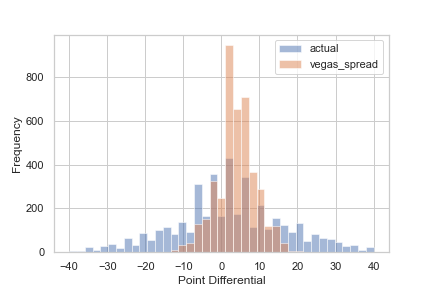
\includegraphics[width = 
 \columnwidth]{figs_final/vegas_vs_true.png}
 \captionof{figure}{Distributions of Actual Point Differentials and Vegas Lines}
\label{fig:histogram}
\end{Figure}
% \begin{Figure}
% \centering  
%  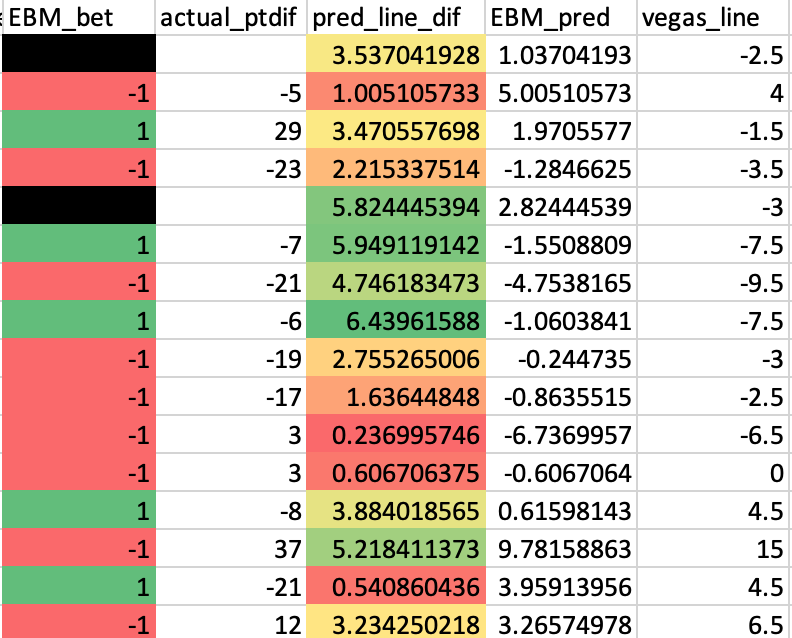
\includegraphics[width = \columnwidth]{figs_final/wk14_2.png}
%  \captionof{figure}{EBM Model Predictions on 2020 Week 14 Games. In the left-most column, green cells correspond to bets that would have won following the guidance of the EBM model, and red cells indicate bets that would have lost. Black cells indicate the game has not yet occurred. The third column from the left serves as a visualization of how far the EBM prediction is from the Vegas line. Green cells indicate large difference, and red cells indicate small difference.}
% \label{fig:wk14}
% \end{Figure}
\subsection{Modeling on SAO Dataset}
We shuffled and split the dataset with an 80:20 train:test ratio which we hypothesized would supply enough data for training a strong model while leaving enough data to accurately evaluate and validate the model. We standardized the features in the train and test set using the standard deviation and mean from our training set. We standardized both sets with the standard deviation and mean from the training set because when our model encounters new data, it will only have access to these metrics for the data it trained on, so this best simulates how the model will process new data. This ensured that all of our features followed a normal distribution with 0 mean and a standard deviation of 1.  This was necessary because our features did not lie on the same scale, such as win percentage [0,1] and passing yards per game [0,400+]. Without standardization, large variations in a statistic with larger scale like passing yards can dominate the model.

First, we built a linear regression model. The mean absolute error on our train set and test set were 10.86 and 10.70, respectively.  This error was already close to the error of Vegas lines, but we wanted to see if we could get better results using ridge and lasso regressions. With ridge regression, we saw mean absolute error on our train set and test set were 10.86 and 10.69, respectively. With lasso regression, we observed mean absolute error on our train set and test set were 10.87 and 10.70, respectively. We performed cross-validation to optimize the weight (alpha value) applied to the regularization factors. Once performing RidgeCV and LassoCV predictions we were able to slightly improve our predictions for both by a marginal amount. The performance of these initial models still was not as close as we wanted to get to the performance of Vegas lines.

To try to improve our results, we decided to abandon the assumption that our features and the game’s point differential had a linear relationship. Our next idea was to run an Explainable Boosting Machine (EBM) model from Microsoft’s InterpretML module, since this model would be easy to interpret, more flexible in fitting the data, and regularizes the predictor functions to avoid overfitting. EBM models have the advantage over linear models of not being restricted to linear relationships between the features and the prediction space; instead, EBM models fit a smooth curve to each feature. This was the model that performed the best with a train and test set mean error of 10.62 and 10.68, respectively. This was very promising to see, but nonetheless our mean error from the EBM model was still larger than the Vegas prediction.
\subsection{Modeling on SAM Dataset}
In order to place emphasis on a team’s recent performance in predicting the outcome of a game, we next built models with the SAM dataset which incorporated moving averages over a 2-game window in addition to season averages. We ran the same simple linear regression model as well as ridge, lasso, and EBM models on our new dataset. When we ran these models we had test set mean errors that were significantly larger than they were previously, and significantly larger than the training set mean errors.

We suspected this severe overfitting to be attributable to the high correlation between season average statistics and statistics over the past two games. We visualized the correlation between features using a feature correlation matrix, and found that many of the features were highly collinear. In particular, each feature in the moving average was highly correlated to the corresponding feature in the season average as visualized by the orange diagonal lines observable in the appendix figure. It was clear we were overfitting with these models and would need to do more feature engineering to avoid this problem. 

At this point in our analysis, we decided to direct our focus to analyzing results of the models built using the SAO dataset rather than trying to perform further feature engineering with the SAM dataset.
\section{Results}
\subsection{Predictions vs Vegas 2018-2019}
Now that we had some models we were more confident in, we started the process of comparing our results with Vegas. However, we soon came across a fallacy in our training of past data. We realized that an 80:20 split is not realistic for training and testing as the model would have access to future data during training. In order to run proper evaluations, we would need to split our train and test data so that nothing in the training set came after a game in the test set. We would not be able to randomly shuffle data into our training and test sets as we had previously. We decided to train on all games from 2002 through 2017, with the goal of testing our results on the 2018 and 2019 regular season games. We had some surprising results.

Across all games in 2018 and 2019 we would have won 54.6\% of the time if we placed a bet following the predictions of our model.
\begin{center}
\begin{tabular}{ c c c }
 \toprule
  & \bf Train & \bf Test  \\
 \midrule
 \bf Linear Reg. & 10.66 & 10.86 \\ 
 \bf Ridge Reg. & 10.61 & 10.86 \\ 
 \bf Lasso Reg. & 10.58 & 10.88 \\ 
 \bf EBM & 10.62 & 10.52 \\ 
 \bottomrule
\end{tabular}
\end{center}
\subsection{Predictions vs Vegas 2020 Week 14}


To experiment with the model how it would function in deployment, we tried predicting on the upcoming week 14 games of the 2020 season played on Sunday, Dec. 13th. We trained our model on all regular season games in our SAO dataset from 2002 through 2018. Our model did not do well with this small sample size, predicting correctly on only 4 of 15 games. We did notice that our model seemed to be performing better with games where the difference between our predicted spread and the Vegas line was large. These results are visualized in Figure \ref{fig:wk14}.

\begin{Figure}
\centering  
 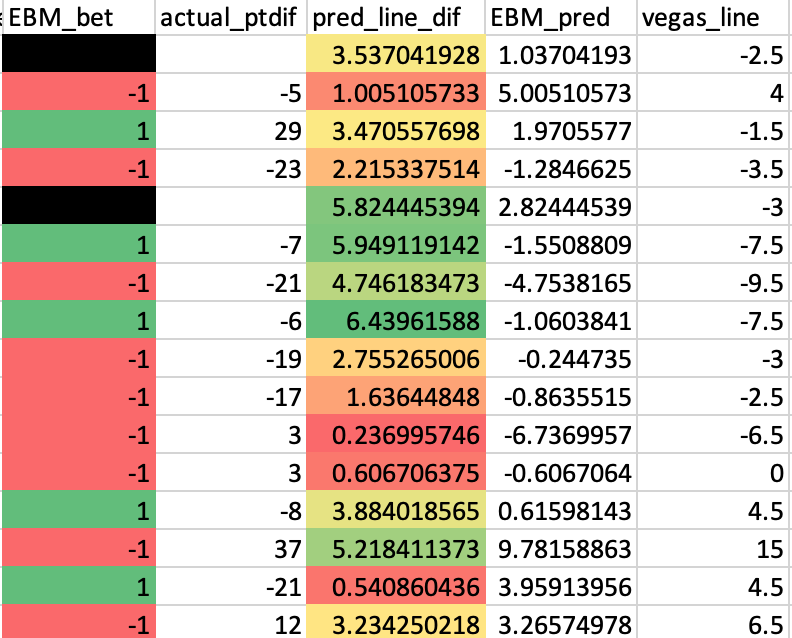
\includegraphics[width = \columnwidth]{figs_final/wk14_2.png}
 \captionof{figure}{EBM Model Predictions on 2020 Week 14 Games. In the left-most column, green cells correspond to bets that would have won following the guidance of the EBM model, and red cells indicate bets that would have lost. Black cells indicate the game has not yet occurred. The third column from the left serves as a visualization of how far the EBM prediction is from the Vegas line. Green cells indicate large difference, and red cells indicate small difference.}
\label{fig:wk14}
\end{Figure}

\section{Discussion}
After analyzing our results, we considered whether our project might produce a Weapon of Math Destruction. We concluded that there could be some scenarios where this model ends up performing so well that it could influence how large swaths of people bet, and thus moves the lines. Moreover, if someone becomes too reliant on our model’s predictions, they might heavily invest in its performance over time and lose significant amounts of money. 

In terms of fairness, similar to other sports prediction models, our model is fair because everyone has access to all of the necessary data that we use to predict point differentials. Moreover, we do not require the use of potentially discriminatory proxies because all of our data is sports statistics scraped from online. Thus, we can continue adapting our model and using this data to predict games in the future without worrying about illegally or unfairly hurting individuals or groups. 
\section{Conclusion}
We are optimistic that our work will encourage the development of new NFL game prediction models. Through some feature engineering we could potentially build an EBM model on our SAM dataset that predicts NFL point differentials more accurately than our EBM model on the SAO dataset. We would need to account for the high collinearity of the features in the SAM dataset to limit the amount of overfitting on SAM. 

Moreover, we could incorporate previous matchup data between two opponents to supplement the moving and season averages. While this could add more relevant features for prediction, it is important to note that additional features could also lead to more overfitting, as we saw when we added moving average features. 

Regardless of potential improvements from feature engineering or model selection on this dataset, we still may not predict as accurately as Vegas’ model simply because we lack the same quantity of information for a better prediction of a football game’s point differential than what they have. We would need to include features such as injured players, quarterback rating, weeks of rest, weather, traveling distance and other miscellaneous factors that could impact a game's outcome.

Our results indicate that if we currently use the EBM model on our SAO dataset to place bets against Vegas we will have a 2.2 percent edge;  we calculate this by finding the difference in our models performance, 54.6 percent, and the break even point against Vegas’ spreads, 52.4 percent. 
\section*{Acknowledgments}
We would like to thank the reviewers that raised Github issues with feedback, and Professor Madeleine Udell for all of her hard work putting together ORIE 4741: Learning with Big Messy Data
\section*{References}
Explanation & Interpretability: InterpretML: Explainable Boosting Machines (EBMs) Guest Lecture for ORIE 4741, Rich Caruana, Senior Principal Researcher at Microsoft,
\href{https://www.legalsportsbetting.com/how-much-money-do-americans-bet-on-sports/}{\underline{Legal Sports Betting}},
\href{https://www.pro-football-reference.com/teams/buf/2019.htm}{\underline{Pro Football Reference}}
\pagebreak
\end{multicols}

\section{Appendix}
\begin{figure}[h!]
\centering 
 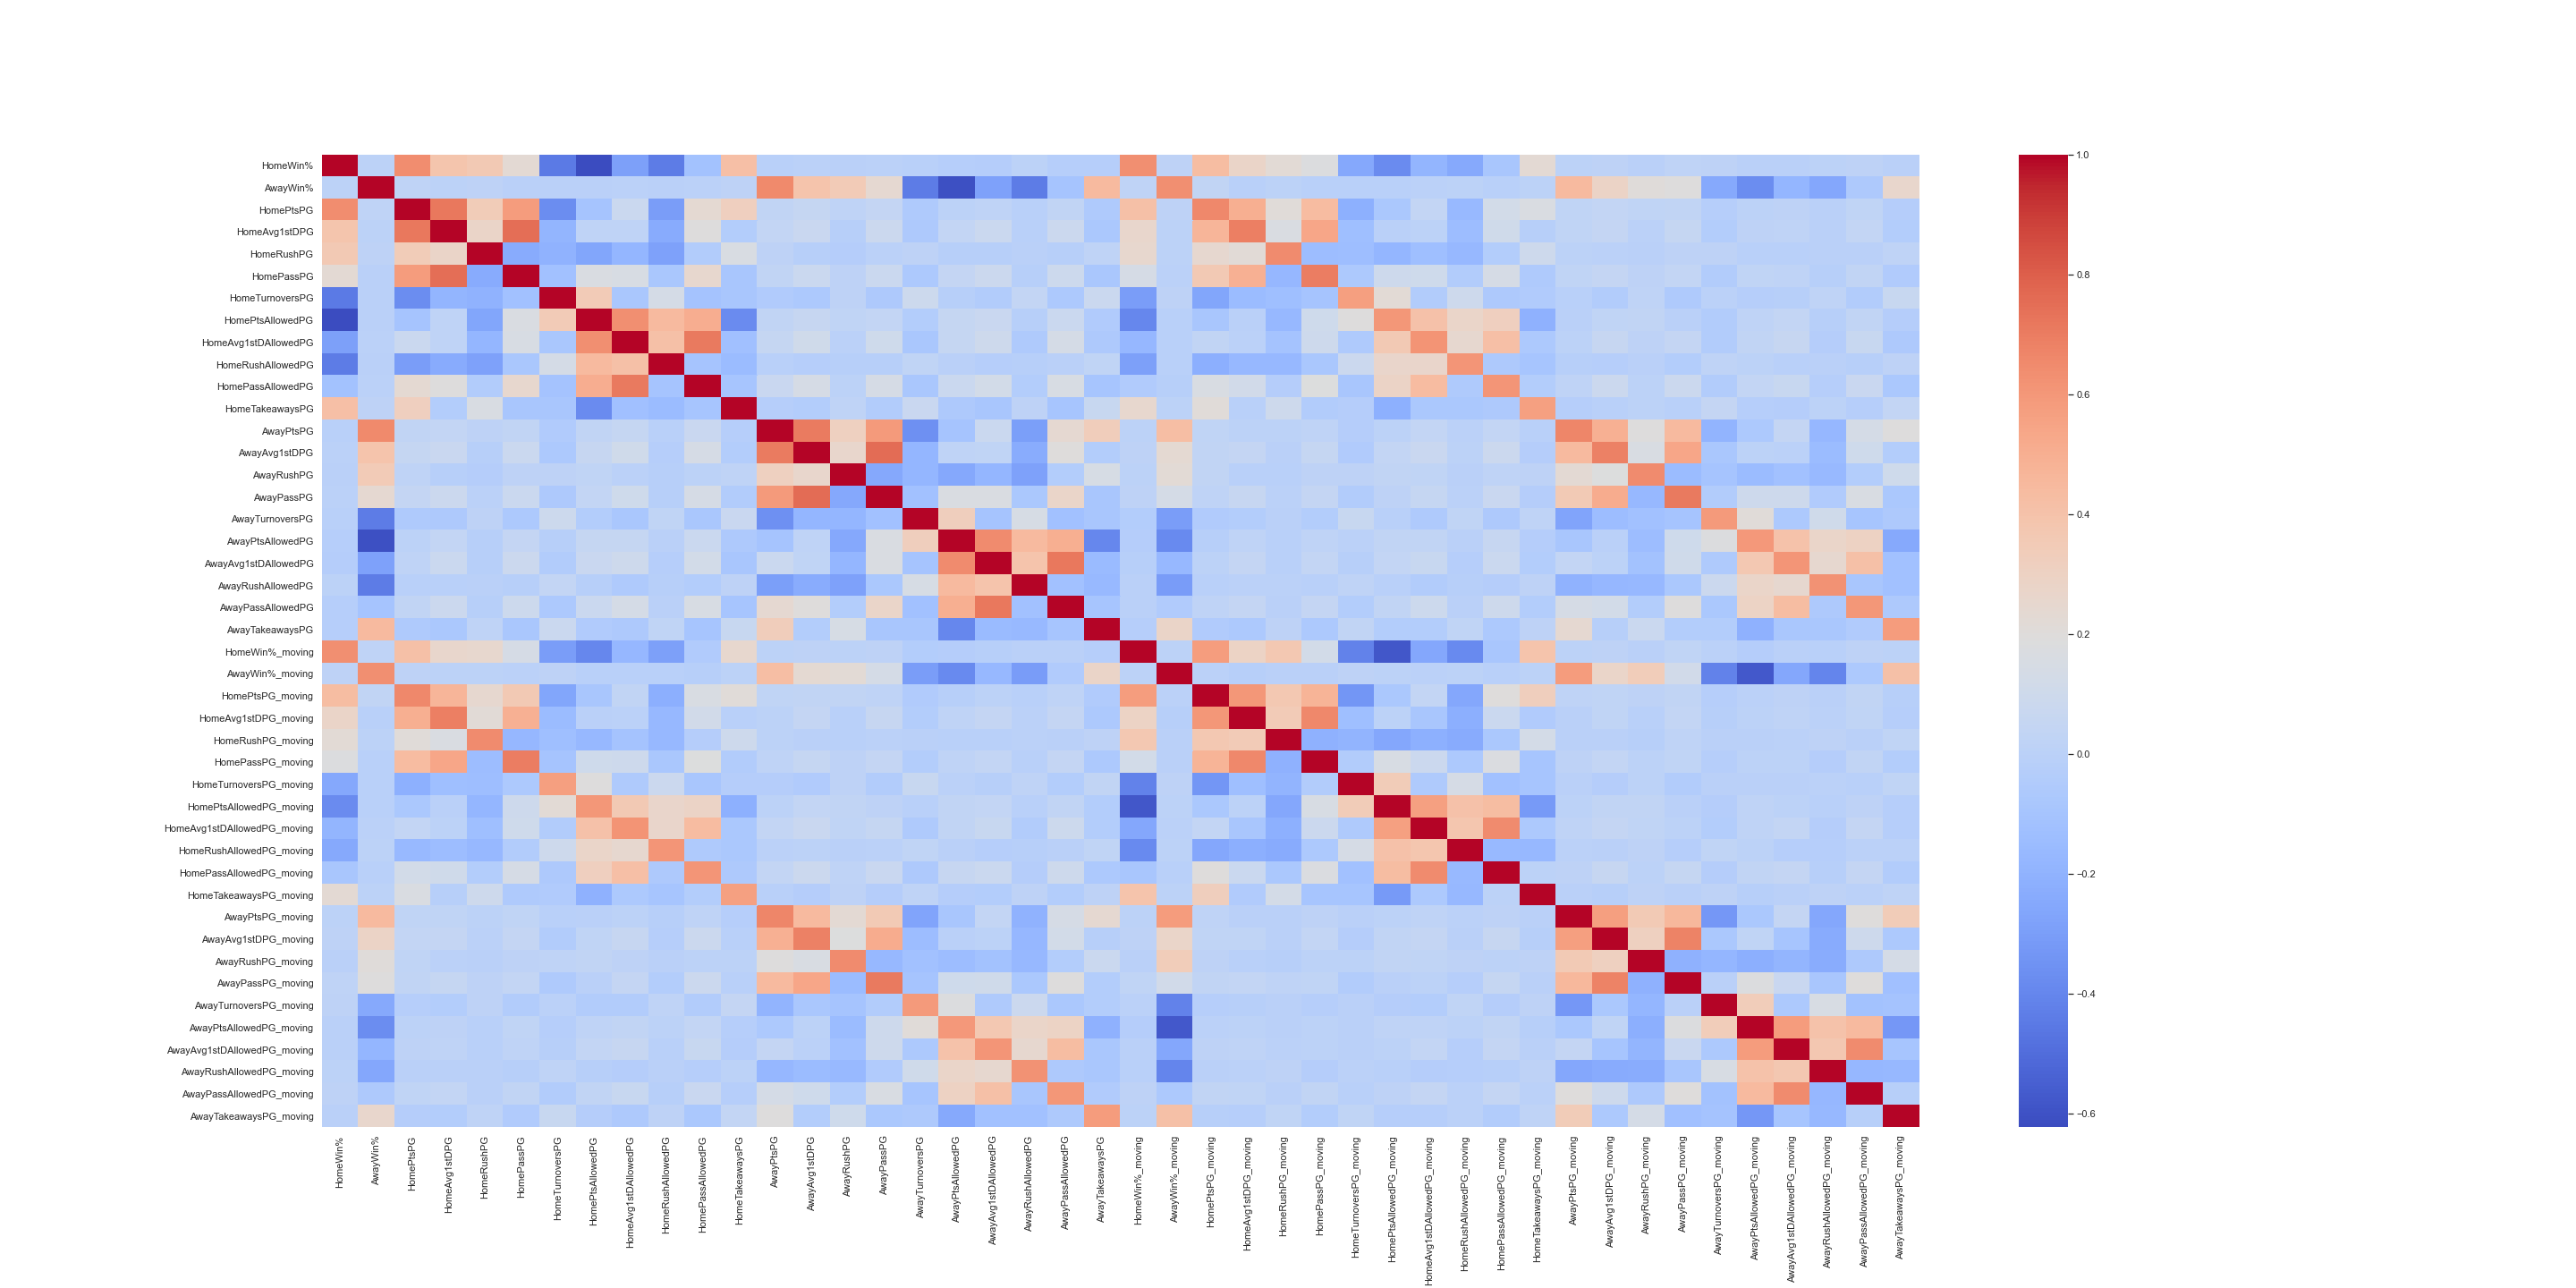
\includegraphics[width=\linewidth]{figs_final/heat_map.png}
 \caption{NFL Game by Game Feature Correlation Matrix}
\label{fig:real}
\end{figure}
\end{document}
